\documentclass{IOS-Book-Article}

\usepackage{cite}
\usepackage{mathptmx}

\usepackage[pdftex]{graphicx}
% declare the path(s) where your graphic files are
% \graphicspath{{../pdf/}{../jpeg/}}
% and their extensions so you won't have to specify these with
% every instance of \includegraphics
\DeclareGraphicsExtensions{.pdf,.jpeg,.png}

\usepackage{url}

\def\hb{\hbox to 10.7 cm{}}

\newcommand{\psykal}{{PS}y{KA}l\ }

\begin{document}

\pagestyle{headings}
\def\thepage{}

\begin{frontmatter}              % The preamble begins here.
%
% paper title
% can use linebreaks \\ within to get better formatting as desired
\title{Towards Compiler-Agnostic Performance in Finite-Difference Codes}

\author[A]{\fnms{A. R.} \snm{Porter}%
\thanks{Corresponding Author: Andrew Porter, STFC Daresbury Laboratory, Warrington, WA4 4AD, UK; E-mail:
andrew.porter@stfc.ac.uk.}},
\author[A]{\fnms{R. W.} \snm{Ford}},
\author[A]{\fnms{M.} \snm{Ashworth}},
\author[A]{\fnms{G. D.} \snm{Riley}}
and
\author[B]{\fnms{M.} \snm{Modani}}
\runningauthor{A.~R.~Porter et al.}
\address[A]{STFC Daresbury Laboratory, Warrington, WA4 4AD, UK}
\address[B]{IBM India}

\begin{abstract}
In this paper we evaluate the performance implications of applying a
technique called \psykal to finite difference Ocean models. 
%
In \psykal, the code related to the underlying science is formally
separated from code related to parallelisation and single core
optimisations. This separation of concerns allows scientists to code
their science independently of the underlying hardware architecture
(thereby keeping a single code base) and for optimisation specialists
to be able to tailor the code for a particular machine independently
of the science code.
%
A finite difference shallow water benchmark optimised for cache based
architectures is taken as the starting point. A vanilla \psykal version
is written and the performance of the two compared. The optimisations
that were applied to the original benchmark (loop fusion etc) are then
applied to the \psykal version as a set of code modifications to the
optimisation layer. Performance results are presented for the Cray,
Intel and GNU compilers on Intel Ivybridge and Haswell processors and
for the IBM compiler on Power8.
%
Results show that the combined set of code modifications obtain
performance that is within a few percent of the original code for all
compiler and architecture combinations on all tested problem sizes
apart from GNU on Haswell, one problem size for Intel on Haswell and
IBM on Power8.
%
As the GNU compiler performs well on Ivybridge the reduction in
performance for the \psykal version was not analysed further. As the
Intel performance on Haswell was better for the \psykal version than
the original version, it was not analysed further.
%
In the case of the IBM compiler, the \psykal performance is
significantly better than the original hand optimised code on all
problem sizes. Analysing the performance of the IBM compiler shows
that a different structure for the original optimised code produces
much improved performance. Replicating this different structure using
appropriate transformations in the \psykal version provides the
same performance improvements.
%
Therefore, the \psykal approach can be used with negligable
performance loss and sometimes small performance gains compared to the
original optimised code, there is no single best hand optimised
implementation of the code for all the compilers tested, and the
flexibility in applying code modifications to the optimisation layer
in the PSyKAl version allows for a significant performance improvement
on the IBM Power8 compared with the original code.

\end{abstract}

\begin{keyword}
Performance, Code-generation, Finite-difference
\end{keyword}

\end{frontmatter}

%%%%%%%%%%%%%%%%%%%%%%%%%%%%%%%%%%%%%%%%%%%%%%%%%%%%%%%%%%%%%%%%%%%%
% Introduction is not to be numbered so use \section*{}
\section*{Introduction}
The challenge presented to the developers of
scientific software by the drive towards Exascale computing is
considerable. With power consumption becoming the overriding design
constraint, CPU clock speeds are falling and the complex,
multi-purpose compute core is being replaced by multiple, simpler
cores. This philosophy can be seen at work in the rise of so-called
accelerator based machines in the Top 500 List~\cite{top500} of
supercomputers: five of the top-ten machines in the November 2014 list
make use of Intel Xeon Phi's or NVIDIA GPUs. Four of the remaining
five machines in the top ten are IBM BlueGene/Qs, the CPU of which has
hardware support for running 64 threads.

Achieving good performance on large numbers of light-weight cores
requires exploiting as much parallelism in an application as possible
and this results in increased complexity in the programming models
that must be used. This in turn increases the burden of code
maintenance and code development, in part because two specialisms are
required: that of the scientific domain which a code is modelling
({\it e.g.} oceanography) and that of computational science. The
situation is currently complicated still further by the existence of
competing hardware technology; if one was to begin writing a major
scientific application today it is unclear whether one would target
GPU, Xeon Phi, traditional CPU, FPGA or something else entirely. This
is a problem because, generally speaking, these different technologies
require different programming approaches.

\subsection{The \psykal Approach}

%Proliferation of lightweight cores is resulting in increased
%complexity in the programming models required to achieve performance.
%Combine with the complexity of e.g. a model simulating circulation in
%the global ocean. Significant challenge in software engineering.
%Propose an approach for meeting this challenge by separating the
%computational science demands from the {\it e.g.} oceanographic
%demands.

The \psykal approach separates code into three layers; the Algorithm
layer, the PSy layer and the Kernel layer. While this approach is
general, we are currently applying it to Atmosphere and Ocean models
written in Fortran where domain decomposition is typically performed
in the latitude-longitude direction, leaving columns of elements on
each domain-decomposed partition.

The top layer, in terms of calling hierarchy, is the Algorithm
layer. This layer specifies the algorithm that the scientist would like
to perform (in terms of calls to kernel and infrastructure routines)
and logically operates on full fields. We say logically here as the
fields may be domain decomposed, however the algorithm layer is not
aware of this. It is the scientist's responsibility to write this
algorithm layer.

The bottom layer, in terms of calling hierarchy, is the Kernel
layer. The Kernel layer implements the science that the Algorithm
layer calls, as a set of subroutines. These kernels operate on local
fields (a set of elements, a single column of elements, or a set of
columns, depending on the kernel). Again the scientist is responsible
for writing this layer and there is no parallelism specified here,
but, depending on the complexity of the Kernels, there may be input
from an HPC expert and/or some coding rules to help ensure the kernels
compile into efficient code.

The PSy layer sits in-between the Algorithm and Kernel layers and its
functional role is to link the algorithm calls to the associated
kernel subroutines. As the Algorithm layer works on logically global
fields and Kernel layer works on local fields, the PSy layer is
responsible for iterating over columns. It is also responsible for
including any required distributed-memory operations, such as halo
swaps and reductions.

As the PSy layer iterates over columns, the single core performance
can be optimised by applying transformations such as loop fusion and
loop blocking. Additionally, the potential parallelism within this
iteration space can also be optimised and parallelised. The PSy layer
can therefore be tailored for a particular hardware (such as
multi-core, many-core, GPGPUs, or some combination thereof) and
software (such as compiler, operating system, MPI implementation)
configuration with no change to the algorithm or kernel layer
code. This approach therefore offers the potential for portable
performance.

Clearly the separation of code into distinct layers may have an effect
on performance. This overhead, and how to get back to the performance
of a hand optimised code, and potentially improve on it, will be
discussed in the remainder of this paper.

\subsection{The `Shallow' Program}

For this work we use a benchmark called Shallow which solves the
shallow-water equations on a bi-periodic plane following the
finite-difference scheme introduced by Sadourny~\cite{sadourny75}.
This software was originally written in 1984 by Paul Swarztrauber of
the National Center for Atmospheric Research, US.  However, in common
with many scientific codes, it has subsequently undergone some sort of
evolutionary development with subsequent people making various changes
and optimising it for previous generations of hardware.  In describing
our work, we term the version of the Shallow program obtained at the
beginning of this project the `original' version.

Shallow is a very good test case for our purposes since the original
version is short (some 600 lines) and contained within a single source
file. This makes it relatively straightforward for a compiler to
optimise. Its performance is thus quite a demanding target for our
modified versions of the code to reproduce.

Since any real oceanographic computational model must output results,
we ensure that any \psykal version of Shallow retains the Input/Output
capability of the original. This aids in limiting the optimisations
that can be performed on the \psykal version to those that should also
be applicable to full oceanographic models. Note that although we
retain the I/O functionality, all of the results presented in this work
carefully exclude the effects of I/O since it is compute performance
that interests us here.

In order to maximise the flexibility (and thus potential for
optimisation) of the \psykal version of Shallow, we made the kernels
as fine-grained as possible. In this case, this resulted in eight
distinct kernels, each of which operated on a single field at a single
point (since we have chosen to use point-wise kernels). With a little
bit of tidying/re-structuring, we found it was possible to express the
contents of the main time-stepping loop as a single invoke (a call to
the PSy layer) and a call to the I/O system
(Figure~\ref{FIG_psykal_shallow_structure}). The single PSy-layer
routine then consists of applying each of the kernels to all of the
points on the model mesh requiring an update. In its basic,
unoptimised (`vanilla') form, this PSy-layer routine then contains a
doubly-nested loop around each kernel call, as indicated by the
pseudo-code in Figure~\ref{FIG_psykal_shallow_structure}.

\begin{figure}
\centering
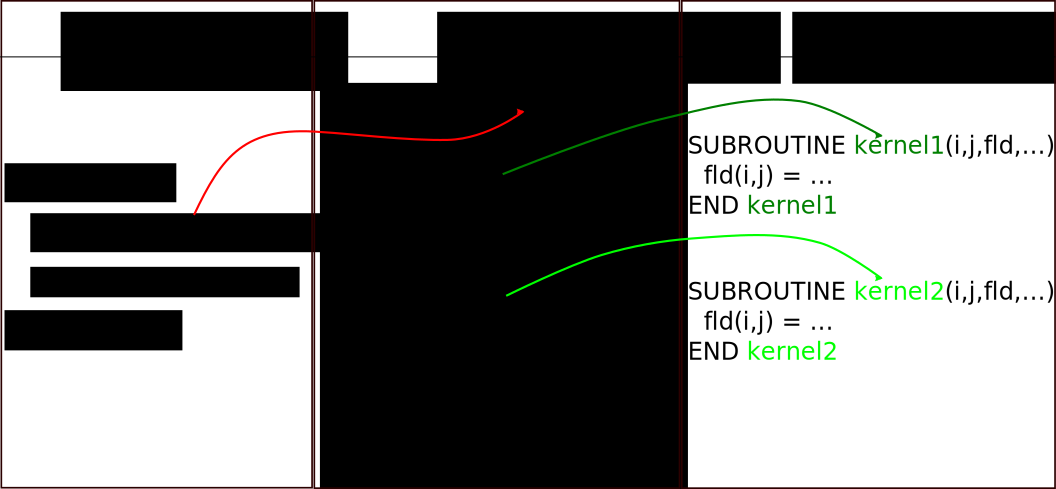
\includegraphics[width=85mm]{psykal_shallow}
\caption{A schematic of the vanilla \psykal version of the Shallow code.}
\label{FIG_psykal_shallow_structure}
\end{figure}

As with any full oceanographic model, boundary conditions must be
applied at the edges of the model domain. In the case of Shallow we
have periodic boundary conditions in both the $x$ and $y$ dimensions.
These are simply implemented by having additional (`halo')
rows/columns at the edges of the domain and ensuring the data in them
is up-to-date before it is read. These rows/columns are updated by
copying data from the corresponding row/column on the opposite side of
the domain. In the current work, the lines of code to do these copies
is manually inserted in the PSy-layer routine as required.

%{\bf Auto-generated BC code by reasoning about meta-data. But then,
%  that brings us on to meta-data...}

%%%%%%%%%%%%%%%%%%%%%%%%%%%%%%%%%%%%%%%%%%%%%%%%%%%%%%%%%%%%%%%%%%%%
\section{Methodology(?)}

The primary aim of this work is to determine whether any performance
loss due to the \psykal separation of concerns can be negated by
optimising the PSy layer. To evaluate this we perform tests on a range
of hardware and a range of compilers. The hardware and compilers are
listed in Table~\ref{TABLE_compilers}. Where a compiler is available
on a given piece of hardware, the version number used in this work is
specified.
%
The Intel Haswell-based system (Xeon E5-1620 v2) has a clock speed of
3.7~GHz and 10~MB of last-level cache. The Intel Ivy Bridge-based
system (Xeon E5-2697) has a clock speed of 2.7~GHz and a last-level
cache of 30~MB. The CPU in the IBM Power-8 system is built around 12
'chiplets'. Each chiplet has a single core with 64~KB of L1 cache,
512~KB of L2 cache and 8~MB of L3 cache. The L3 cache of each chiplet
is shared with all other chiplets so that there is a total of 96~MB of
last-level cache. The cores on the system we used had a clock speed of
3.3~GHz.

\begin{table}[!t]
% increase table row spacing, adjust to taste
\renewcommand{\arraystretch}{1.3}
\caption{The matrix of compilers and CPUs used in this work. The use
  of a compiler on a given CPU is indicated by the specification of
  the version of the compiler in the relevent element. No entry
  indicates that a compiler was not available/used on that CPU.}
\label{TABLE_compilers}
\centering
\begin{tabular}{|l|c|c|c|c|}
\hline
                 & \multicolumn{4}{c|}{Compiler}             \\
\hline
                 & Gnu   & Intel       & Cray    & IBM     \\
\hline
Intel Haswell    & 4.8.2 & 14.0.0      &         &          \\
Intel Ivy Bridge & 4.9.1 & 14.0.1.106  & 8.3.3   &          \\
IBM Power 8      &       &             &         & 15.1.2     \\
\hline
\end{tabular}
\end{table}

In Table~\ref{TABLE_compiler_flags} we give the optimisation flags
used with each compiler. These flags are particularly important for
the \psykal versions of the code. The performance of the original
version of the code is much less sensitive to the compiler
options. This is because it consists of a single source file
containing effectively a single routine (excluding those for I/O).
 
\begin{table}[!t]
% increase table row spacing, adjust to taste
\renewcommand{\arraystretch}{1.3}
\caption{The compiler flags used in this work.}
\label{TABLE_compiler_flags}
\centering
\begin{tabular}{l|l}
\hline
Compiler  &  Flags \\
\hline
Gnu       & -Ofast -mtune=native -finline-limit=50000    \\
Intel     & -O3 -fast -fno-inline-factor    \\
Cray      & -O3 -O ipa5 -h wp               \\
IBM       & \parbox{5cm}{-O5 -qinline=auto:level=10\\ -qinline=auto:level=10 -qaltivec=be\\ -qdebug=NSIMDUBTHRESHOLD -qprefetch=dscr=0x1D7} \\
\hline
\end{tabular}
\end{table}

Before applying any code transformations, we benchmark the original
version of the code. We also benchmark the vanilla, unoptimised
version after it has been re-structured following the \psykal
approach. These two versions of the code effectively provide upper and
lower bounds, respectively, on the performance we expect to achieve.

{\bf RF: Explain that we gradually apply transformations which restructure the psykal code to end up with the same optimised structure as the original code. Explain the reason behind the ordering and what each does - I think you said it was the order that you thought would make the biggest difference. If you can base it on performance analysis then all the better but I don't think that is required.}

{\bf Performance analysis as motivation for the code
  tranformations. More detail on each transformation.}

Beginning with the vanilla \psykal version, we then apply a series of
code transformations while obeying the \psykal separation of concerns,
{\it i.e.} optimisation is restricted to the middle, {PS}y layer and leaves
the kernel and algorithm layers unchanged. The aim of these
optimisations is to recover, as much as is possible, the structure and
thus performance of the original version of the code. The
transformations we have performed are as follows:
\begin{enumerate}

\item Pass explicit array bounds to middle layer (rather than using
  assumed-size array arguments)

\item Move kernel routines into same module as middle layer

\item Loop fusion

\item In-lined field-copy operation

\item Fused field-copy operation

\item Manually in-line kernel bodies into middle-layer code

\item Fully fuse first loop (only the outer loop of this loop nest was
  fused in the first pass)

\item Make the array/loop bounds explicitly constant for the
      duration of the time-stepping loop.
\end{enumerate}

We shall see that these transformations do not always result in improved
performance. Whether or not they do so depends both on the compiler
and the problem size. We also emphasise that the aim of these
optimisations is to recover, as far as is possible, the structure of
the original version of the code. It may well be that transforming the
code into some other structure would result in better performance on a
particular architecture. However, exploring this optimisation space is
beyond the scope of the present work.

We explore the extent to which performance depends upon the problem
size by using square domains of dimension 64, 128, 256, 512 and
1024. This range allows us to investigate what happens when cache is
exhausted as well as giving us some insight into the decisions that
different compilers make when optimising the code.

%%%%%%%%%%%%%%%%%%%%%%%%%%%%%%%%%%%%%%%%%%%%%%%%%%%%%%%%%%%%%%%%%%%%
\section{Results}

In Figure~\ref{FIG_orig_perf_summary} we plot the performance of the
original version of the Shallow code for the range of compilers and
hardware considered here. This summary demonstrates the effect of the
larger last-level cache of the Intel Ivy Bridge system compared to
that of the Haswell system; note the significant drop in performance
in going from a problem size of $256^{2}$ to a problem size of
$512^{2}$ for the black and green bars. The performance of the Ivy
Bridge system with the Cray or Intel compiler (red and purple bars)
only drops to this level when the domain size is increased to
$1024^{2}$. At this point, the working set no longer fits within cache
and performance is dominated by the bandwidth to main memory, making
it relatively insensitive to the choice of compiler. The IBM Fortran
compiler for Linux on Power 8 is relatively immature and failed to
SIMD-vectorise two of the three major loop nests in the time-stepping
loop. Figure~\ref{FIG_orig_perf_summary} therefore also includes the
performance results obtained after the source had been modified to
work-around this limitation (we fissioned one loop nest and manually
unrolled another). Work is currently underway on updating the compiler
so that these modifications will be unecessary with a future release.

\begin{figure}[!t]
\centering
\includegraphics[width=2.8in]{orig_summary}
\caption{Summary of the performance of the original Shallow code on
  the range of compilers and hardware under consideration. *After code
  modifications to encourage SIMD vectorisation (see text).}
\label{FIG_orig_perf_summary}
\end{figure}

For this compiler-friendly form of the code, there is little
performance difference between the executables produced by the Gnu and
Intel compilers. However, the executable produced by the Cray compiler
generally performs significantly better for all but the largest domain
size.

Moving now the to the \psykal version of Shallow,
Figure~\ref{FIG_best_psykal_perf_summary} plots the performance of the
fastest \psykal version for each of the compiler/CPU combinations. The
only significant difference between this and the plot of the
performance of the original version of the code in
Figure~\ref{FIG_orig_perf_summary} is that the difference between the
Gnu- and Intel-compiled executables is slightly more marked. This is
clarified in Figure~\ref{FIG_slowdown_summary} which plots the
percentage difference between the performance of the original and the
(best) \psykal versions of Shallow for each compiler/CPU combination.
It is clear from this plot that the difference in the performance of
the Gnu- and Intel-compiled excutables on the Haswell system is due to
the Gnu compiler being unable to recover the performance achieved by
the original code. In contrast there is no such problem for the
Gnu-compiled executable on the Ivy Bridge system. We attribute this to
the more recent version of the compiler on the latter system (4.9.1 as
opposed to 4.8.2).

\begin{figure}[!t]
\centering
\includegraphics[width=7.5cm]{best_psykal_summary}
\caption{Summary of the best performance achieved by any \psykal 
version of Shallow with each of the compilers and CPUs under 
consideration.}
\label{FIG_best_psykal_perf_summary}
\end{figure}

\begin{figure}[!t]
\centering
\includegraphics[width=2.8in]{slowdown_summary}
\caption{Comparison of the performance of the best \psykal
version with that of the original version of the code. A negative value 
indicates that the \psykal version is faster than the original.}
\label{FIG_slowdown_summary}
\end{figure}

In fact, for the Gnu and Cray compilers on the Ivy Bridge system, the
\psykal version of Shallow is never more than 2\% slower than the
original and in some cases is faster.  This demonstrates that we can
reliably recover the performance of the original version of the code,
despite the significant restructuring required by the \psykal
approach.

The most striking feature of Figure~\ref{FIG_slowdown_summary} is the
fact that the best \psykal version of Shallow is consistently faster
than the original on the Power 8. This confirms that this early
version of the IBM compiler struggled with the original form of the
Shallow source code.

Having shown that, in general, we can recover and occasionally improve
upon the performance of the original version of Shallow, the next
logical step is to examine the necessary code transformations.  We do
this for the $256^{2}$ case since this fits within last-level cache on
all of the CPUs we are using here.  Table~\ref{TABLE_opt_breakdown}
shows detailed timings for this case after each transformation has
been applied to the code. The same data is visualised in
Figure~\ref{FIG_opt_stages_256} where the performance of the \psykal
version for a given compiler/CPU is given relative to the performance
of the original with the same compiler/CPU.

\begin{table*}[!t]
% increase table row spacing, adjust to taste
\renewcommand{\arraystretch}{1.3}
% if using array.sty, it might be a good idea to tweak the value of
% \extrarowheight as needed to properly center the text within the cells
\caption{The mean time-per-step (s) for the $256^2$ case after each 
code transformation.}
\label{TABLE_opt_breakdown}
\centering
\begin{tabular}{l|c|c|c|c|c|c}
\hline
Compiler:          &  Gnu  & Intel   & Gnu & Intel & Cray & IBM \\
\hline
CPU:               & \multicolumn{2}{c|}{Haswell} & \multicolumn{3}{c|}{Ivy Bridge} & Power8 \\
\hline
Original                               &  7.47E-04 & 7.06E-04 &	7.70E-04 & 7.77E-04 & 6.13E-04 &  1.17E-03  \\
Vanilla \psykal                        &  1.26E-02 & 8.64E-04 &	1.38E-02 & 9.82E-04 & 8.33E-04 &  7.87E-03  \\
Explicitly-sized arrays                &  1.26E-02 & 8.62E-04 &	1.38E-02 & 9.65E-04 & 6.96E-04 &  6.74E-03  \\
Kernels copied into module             &  1.10E-03 & 8.67E-04 &	9.42E-04 & 9.65E-04 & 7.10E-04 &  3.13E-03  \\
Loops fused                            &  1.09E-03 & 7.89E-04 &	9.07E-04 & 8.80E-04 & 7.35E-04 &  3.60E-03  \\
In-lined field-copy                    &  1.09E-03 & 7.90E-04 &	9.07E-04 & 8.73E-04 & 7.31E-04 &  3.62E-03  \\
Fused field-copy                       &  1.09E-03 & 9.25E-04 &	1.02E-03 & 1.04E-03 & 6.50E-04 &  4.11E-03  \\
In-line all kernels                    &  8.20E-04 & 7.14E-04 &	9.32E-04 & 8.52E-04 & 6.50E-04 &  1.07E-03  \\
Fully fuse 1st loop nest               &  8.10E-04 & 7.18E-04 &	7.76E-04 & 7.92E-04 & 6.23E-04 &  1.07E-03  \\
Explicit, constant array/loop bounds   &  8.05E-04 & 7.12E-04 &	7.81E-04 & 7.91E-04 & 6.13E-04 &  1.07E-03  \\
Fission new-field update loops         &           &          &          &          &          &            \\
Un-roll time-smoothing                 &           &          &          &          &          &            \\
\hline
\parbox{2.5cm}{\%-slow-down of best {\it c.f.} original} & 7.8 & 0.8 & 0.8 & 1.8 & 0.03 & -9.0    \\
\hline
\end{tabular}
\end{table*}

With the Gnu compiler (first and third clusters in
Figure~\ref{FIG_opt_stages_256}), the vanilla \psykal version of
Shallow only achieves ~5-6\% of the performance of the
original. Simply copying the code for each of the kernel subroutines
into the module from which they are called ('module in-lining') has
the most dramatic effect on the performance of the compiled code; it
now achieves almost 80\% of the performance of the original. The next
most significant transformation is that of manually in-lining the
kernel code itself into the bodies of the loops from which they are
called ('kernel in-lining'). This gets the \psykal version to within
8\% of the performance of the original.  The dramatic performance
improvement obtained from the first transformation demonstrates that
the Gnu compiler is unable to optimise over separate files. Therefore,
the fact that the time-stepping loop in the \psykal version still
retains a call to an I/O routine and a call to the middle-layer, both
of which are in different files, is likely to account for this
remaining performance penalty of 8\%.

With the Intel compiler, the key transformations to recover
performance are different (second and fourth clusters in
Figure~\ref{FIG_opt_stages_256}).  Table~\ref{TABLE_opt_breakdown}
shows that even the vanilla \psykal version of Shallow achieves some
80\% of the performance of the original version. Only two code
transformations were required to increase this to 100\%. The first of
these was the fusion of the computational loops. However, we found
that performance suffered (purple bar) when this was extended to
include the loop required for field copies at the end of a time-step
(Figure~\ref{FIG_time_smooth_code}). Further investigation of this
slow-down revealed that the compiler was unable to SIMD vectorise the
newly-fused loop after it had in-lined the body of the kernel called
from within it. Once this in-lining was done by hand (dark-blue bar),
the compiler was able to vectorise the loop and the performance of the
original version of Shallow was recovered.

\begin{figure}[!t]
\centering
\includegraphics[width=95mm]{opt_stages_256}
\caption{The performance of the \psykal version of Shallow for the
  $256^{2}$ domain at each stage of optimisation. Results are given as
  a percentage of the performance of the original code for each
  compiler/CPU combination. A figure greater than 100\% indicates that
  the \psykal version performs better than the original.}
\label{FIG_opt_stages_256}
\end{figure}

\begin{figure}
\begin{verbatim}
! Time smoothing
DO J=1,N+1
  DO I=1,M+1
    CALL time_smooth_code(i,j,ufld,unew,uold)
!    uold(i,j) = ufld(i,j) + alpha* &
!     (unew(i,j) - 2.*ufld(i,j) + uold(i,j))
  END DO
END DO

! Copy new fields into current fields
DO J=1,N+1
  DO I=1,M+1
    Ufld(I,J) = UNEW(I,J)
  END DO
END DO
\end{verbatim}
\caption{Example of the coding structure that required manual
  in-lining of the kernel body (as indicated by commented-out lines)
  to retrieve the performance of the original version of Shallow with
  the Intel compiler.}
\label{FIG_time_smooth_code}
\end{figure}

The fifth cluster in Figure~\ref{FIG_opt_stages_256} shows the
evolution of the performance of the \psykal version of Shallow with
the Cray compiler. Again, this has significant differences from the
behaviour seen with the Gnu and Intel compilers. As with the Intel
compiler, the performance of the Vanilla \psykal version is fairly
good at 74\% of that of the original. In contrast to the other
compilers consisdered so far, the first significant transformation is
simply to specify the bounds of the arrays being used within the
middle layer using module variables (as opposed to specifying them as
assumed size). This tells the compiler that all of the arrays used in
the middle layer have the same extent and also that all of the
computational loops are over almost all elements of these arrays. This
simple change gives a \psykal version that achieves 88\% of the
performance of the original.

Subsequent transformations actually harm performance until the
field-copy operation of Figure~\ref{FIG_time_smooth_code} is fused
with the preceeding loop. The resulting \psykal version now achieves
94\% of the original performance. Two further steps are required to
match the latter. First, the first loop nest has to be fully fused
(both inner and outer loops fused) and second, the array/loop bounds
are passed as an argument to the middle layer. This is done in order
to specify to the compiler that these bounds remain constant for the
duration of the time-stepping loop.

As with the Gnu compiler, it is module in-lining and kernel in-lining
that are important for the IBM compiler (sixth cluster in
Figure~\ref{FIG_opt_stages_256}). Fusing loop nests actually harms
performance, just as it did for the Cray compiler.

The main conclusion of all this analysis is that while we can employ a
separation of concerns and recover performance, doing so is not
straightforward. Determining how best to optimise even a simple code
such as Shallow is highly compiler- and CPU-dependent. Decisions that
are good on one platform may be bad for another and if these are
written into the source code then they will accumulate over time and
will almost certainly result in a code that does not perform optimally
on any system.

{\bf RF: IBM compiler an example of the above point}

\section{Conclusions}

We have investigated the application of the \psykal separation of
concerns approach to the domain of finite-difference ocean
models. This approach enables the computational science (performance)
related aspects of a computer model to be kept separate from the
natural (oceanographic) science aspects.

As expected, applying this separation of concerns does reduce
performance significantly when comparing with an existing optimised
code. However, the application of code transformations to the
performance/PSy layer and the use of appropriate compiler flags can
recover any performance losses to within a few percent and in some
cases, despite limiting ourselves to transformations which replicate
the structure of the optimised code, result in slightly improved
performance.

The IBM results demonstrate two key points.
%
Firstly, even for a relatively simple
benchmark code, the code structure required to obtain good performance
between different architecture and/or compiler combinations may
differ. For hand optimised codes this implies the need to support
multiple code bases in order to achieve portable performance.
%
Secondly, the \psykal approach directly addresses the problem of
requiring different optimisations for different architectures and/or
compilers by limiting these differences to a separate performance
layer, thereby allowing the natural science code base to remain
unchanged.

In future work we will extend our performance portability analysis of
the \psykal approach to shared memory parallelisation optimisations on
different architectures using different parallalisation techniques (in
particular OpenMP on multi/many-core and OpenACC on GPU's).
%
We will then analyse the performance of a domain specific compiler
that is currently under development. This compiler will generate
optimised PSy-layer code using a user-provided recipe of
transformations, thereby removing the need for optimisation experts to
manually write the PSy layer.

% \bf{Perhaps we don't want to give too much away here so I've removed the optimisation space search plans even though it is mentioned in the text}
% Finally we plan to use this compiler to allow us to search the optimisation sp%ace of transformations to automatically optimise a code for a particular compil%er/architecture combination or to determine whether we can find improved perfor%mance over existing hand optimised solutions and to automatically 


% use section* for acknowledgement
\section*{Acknowledgments}

This work made use of the ARCHER UK National Supercomputing Service
(\url{http://www.archer.ac.uk}). This work was funded by NERC project {\bf xxx}

% http://www.ctan.org/tex-archive/biblio/bibtex/contrib/doc/
\bibliographystyle{unsrt}
% argument is your BibTeX string definitions and bibliography database(s)
\bibliography{shallow_perf}
%
\end{document}


